
%(BEGIN_QUESTION)
% Copyright 2007, Tony R. Kuphaldt, released under the Creative Commons Attribution License (v 1.0)
% This means you may do almost anything with this work of mine, so long as you give me proper credit

Two emergency isolation valves are installed in a process line between two chemical reactor vessels:

$$\includegraphics[width=15.5cm]{i02502x01.eps}$$

These safety shutdown valves normally spend their time in the wide-open position.  Only during emergencies are they expected to close shut.  Two are placed in series so that even if one isolation valve fails to shut when needed there will be another available to do the job.

Suppose the probability of each isolation valve failing on demand (PFD) is equal to 1.5 $\times$ $10^{-4}$, given the age of the valves and actuators, and the frequency of partial-stroke testing.  (Note, the PFD value will be different for valves of different age, and for different testing intervals.)  

Calculate the probability of failure on demand of the two isolation valves {\it together}: the chance that {\it neither} valve will shut when needed during an emergency.  Next, calculate the probability that this isolation system will work properly when needed (i.e. the probability that at least one of the two isolation valves will function properly on demand).

\vskip 20pt \vbox{\hrule \hbox{\strut \vrule{} {\bf Suggestions for Socratic discussion} \vrule} \hrule}

\begin{itemize}
\item{} Does placing two isolation valves in series prioritize {\it dependability} or does it prioritize {\it security}?
\item{} Identify at least one important assumption implicit in the probability calculations shown here.
\end{itemize}


\underbar{file i02502}
%(END_QUESTION)





%(BEGIN_ANSWER)

Since this is a series (double) block valve system, the probability that the safety function fails will be the probability that {\it both} block valves fail to shut on demand.  Thus, the PFD for both valves together = 2.25 $\times$ $10^{-8}$

$$\includegraphics[width=15.5cm]{i02502x02.eps}$$

\vskip 10pt

The probability that this safety function will perform as designed and shut off the flow when needed (i.e. that is will be {\it dependable}) is the complement of its PFD:

$$\includegraphics[width=15.5cm]{i02502x03.eps}$$

\vskip 10pt

An alternative method for calculating the dependability of this system is to begin with the dependability figures for each block valve.  If the PFD for each valve is $1.5 \times 10^{-4}$, then the dependability of each valve (i.e. the probability that it will shut off when it is supposed to) will be the complement of this value, or 0.99985.  Since the dependability of the whole safety function is the probability that either or both of these block valves operates properly, we may model this as an OR function:

$$\includegraphics[width=15.5cm]{i02502x04.eps}$$

\vskip 10pt

Note: if you are having trouble seeing the relationship between individual PFD's and the overall PFD of the system, try simplifying the problem.  Consider each valve to be a 6-sided die, where rolling a ``1'' is equivalent to failing, and rolling anything else (2 through 6) is considered success.  Now calculate the probability of failure for the whole system (i.e. both dice rolling ``1'').

%(END_ANSWER)





%(BEGIN_NOTES)

The probability of success ($P(\hbox{good})$) is the probabilistic complement of the probability of failure on demand (PFD).  That is, 

$$P(\hbox{good}) = 1 - \hbox{PFD}$$

\vskip 10pt

The important assumption implicit in the given answers is that the control logic is fail-proof.  The PFD figure of 2.25 $\times$ $10^{-8}$ for both valves is {\it for the valves alone}.  If you include (add) the PFD for the control logic, the number will of course be larger!

%INDEX% Mathematics, probability: complementation
%INDEX% Safety, system reliability: probability of failure on demand (PFD)
%INDEX% Safety, system reliability: probability of reliable operation

%(END_NOTES)


